\documentclass[12pt]{ctexart}
\usepackage{amsmath,graphicx,textcomp,subfigure,indentfirst,ctex,color,float}
\title{Lecture 7}
\author{赵思逸}

\date{2022年4月12日}

\newcommand{\refeq}[1]{式~(\ref{#1})}
\newcommand{\reffig}[1]{图~(\ref{#1})}
\begin{document}

\maketitle

\section{视界(Horizon)}

\subsection{粒子视界 (partcle horizon)}
粒子视界 (partcle horizon) :对于过去的事件所能观测到的最远距离。或在 $t$ 时刻看到的最远宇宙在 $t$ 时刻的距离。

\begin{equation}
    d_{ph}(t) = a(t) \int_0^t \frac{cdt'}{a(t')} 
\end{equation}

在今天,
\begin{equation}
    d_{ph}(t_0) = \frac{c}{H_0}\int_0^1 \frac{da'}{a'^2 \sqrt{\Omega_R a'^{-4}+\Omega_M a'^{-3}+\Omega_\Lambda+\Omega_K a'^{-2}} }
\end{equation}

\begin{itemize}
    \item 对于辐射为主的宇宙, $a\propto t^{1/2}$, $d_{ph}(t_0)=2t_0 = D_H$.
    \item 对于冷物质为主的宇宙, $a\propto t^{2/3}$, $d_{ph}(t_0)=3t_0 = 2 D_H$. 
\end{itemize}

\subsection{事件视界(event horizon)}
事件视界(event horizon):未来的观测者所能看到的在 $t$ 时刻或以后的事件在 $t$ 时刻的最远距离。

\begin{equation}
    d_{eh}(t) = a(t) \int_t^\infty \frac{cdt'}{a(t')} 
\end{equation}

\begin{itemize}
    \item 对于冷物质为主的宇宙, $a\propto t^{2/3}$, $d_{eh}\to \infty$. 
    \item 若 $\Lambda$ 为主, $a\propto e^{Ht}$ , $H=H_0 \Omega_\Lambda^{1/2}$,  $d_{eh}\to \frac{c}{H}$ 常数,足够时间以后,只有引力束缚的本星系群能看到。 
\end{itemize}

\subsection{}
从  $t$ 时刻发出的信号 在未来 $T$ 时刻所能到达的最远距离
\begin{equation}
    \lim_{T \to \infty}   a(T) \int_t^T \frac{cdt'}{a(t')} = d_{eh} \frac{a(T)}{a(t)}
\end{equation}

若 $\Lambda$ 为主, $a\propto e^{Ht}$ , $H=H_0 \Omega_\Lambda^{1/2}$,  $d_{eh}\to \frac{c}{H}$ 常数,但 $a(T)\to \infty$,所以我们发出的信号可以到达无限远。 

\begin{figure}[!hbtp]
	\centering
	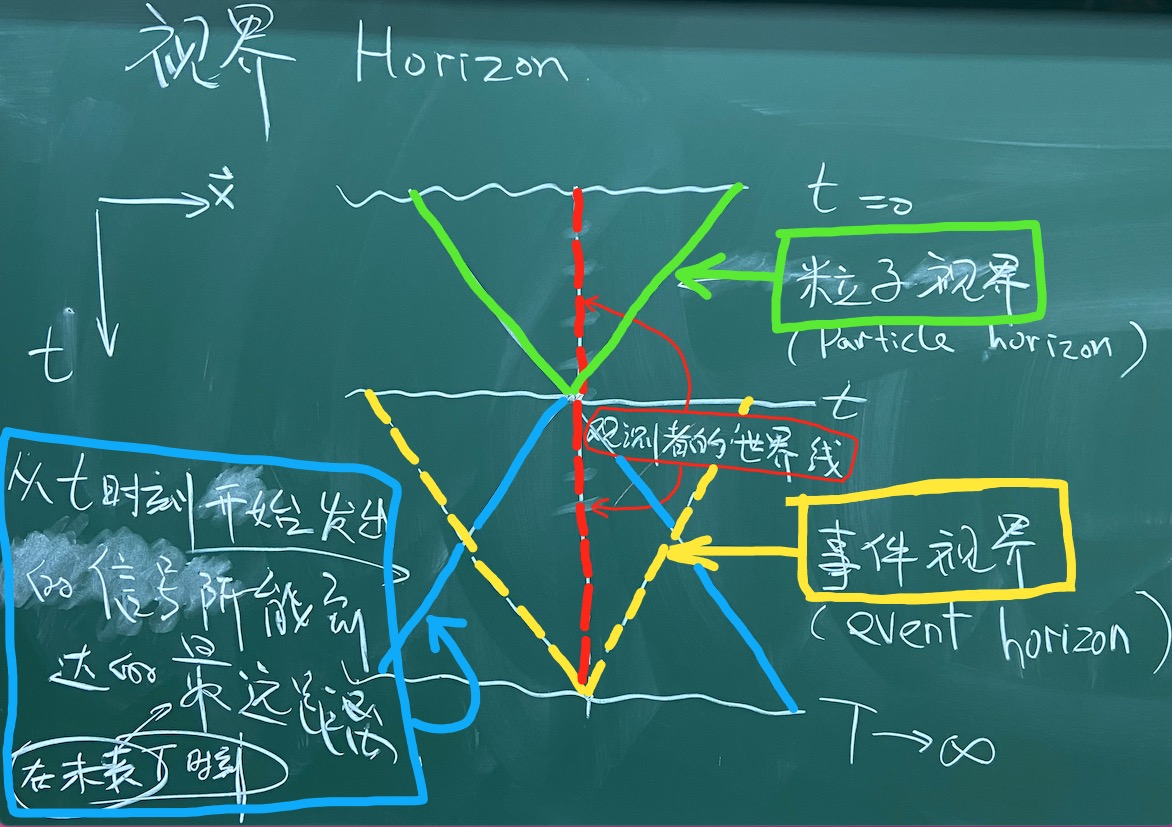
\includegraphics[width=1.0\linewidth]{horizon.jpg}
	\caption{视界}
\end{figure}

\section{早期宇宙的历史}

本章会讲3个重要的话题:
\begin{itemize}
    \item CMB 微波背景辐射
    \item BBN 大爆炸核合成
    \item Inflation 暴涨宇宙
\end{itemize}

\section{微波背景辐射}

\subsection{退耦(decoupling)}

自由质子和自由电子复合成中性氢原子,放出光子(大于等于13.6 eV),中性氢原子也可以吸收光子电离为自由的质子和电子。

随着宇宙膨胀,光子能量降低,复合率逐渐变得远大于电离率。
具体地说,当 $k_B T =0.3 \mathrm{~eV}$ 时,复合率远大于电离率。

另一方面,当光子和电子的散射速率小于宇宙膨胀速率后,光子和电子退耦。

光子被电子散射的速率 $\Lambda_\gamma = \sigma_T n_e v$,其中 $\sigma_T$ 是Thomson散射截面,$n_e$ 是电子数密度, $v$是电子运动速度。早期运动速度接近光速,$\Lambda_\gamma \simeq \sigma_T n_e c \propto a^{-3} \propto \left(T/T_{\gamma 0}\right)^3 $ 其中$T_{\gamma 0}$ 是今天CMB的温度。

宇宙膨胀速率,在辐射占主导期, $H\propto a^{-2} \propto \left(T/T_{\gamma 0}\right)^2$ 。早期散射速率远大于膨胀速率,能达到化学平衡。但散射速率降得更快,当散射速率小于宇宙膨胀速率,化学平衡被打破。

在化学平衡中的等离子体中,光子不断被散射,宇宙对光子是不透明的(opaque),化学平衡被打破时,光子不再发生散射,而是惯性运动,形成最后散射面。最后散射面由被我们观测到的CMB光子的最后一次散射位置组成,近似为一个二维球面。见\reffig{fig.LastScat}

\begin{figure}[!hbtp]
	\centering
	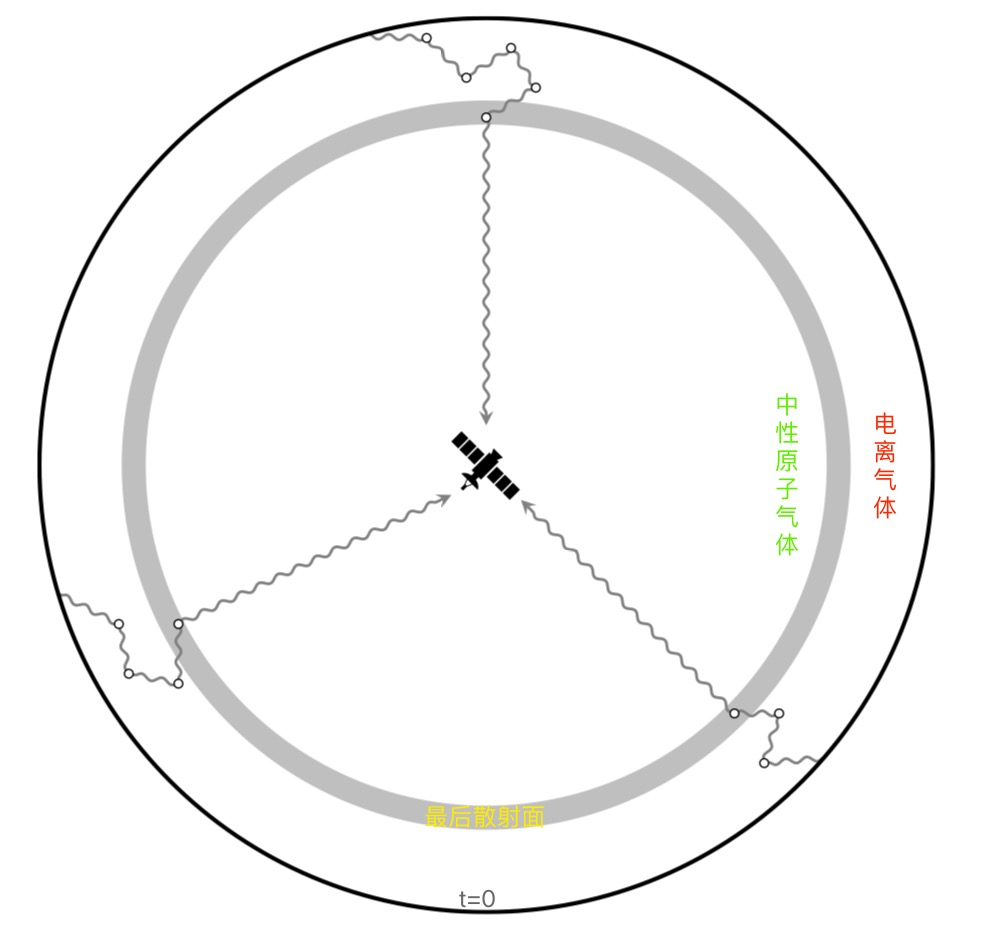
\includegraphics[width=1.0\linewidth]{lastScatter2022.jpg}
	\caption{图中灰色圆环为最后散射面,修改自 Daniel Baumann: Cosmology (2021)} \label{fig.LastScat}
\end{figure}

\subsection{CMB的特征}

\begin{itemize}
    \item 各向同性:来自所有方向的CMB温度高度相同。
    \item 辐射场强度随频率的分布符合黑体辐射谱。(Planck公式)
    \item 退耦能标约为 $0.3\mathrm{eV}$,温度约为3000K,红移约为1100
    \item 温度涨落有偶极矩。(因为地球、太阳、银河系的运动。)
    \item 扣除偶极矩后,仍然存在微小的温度起伏,这就是后来宇宙密度起伏、形成星系等结构的种子/初始条件。
\end{itemize}

为什么CMB符合黑体谱?

在最后散射面 $t_L$,光子辐射谱满足Planck公式:
\begin{equation}
    n_{T(t_L)}(\nu_L) d \nu_L=\frac{8 \pi \nu_L^{2} d \nu_L}{\exp \left(\frac{h_\text{pl} \nu_L}{k_{B} T(t_L)} \right)-1}
\end{equation}
在$t>t_L$,光子频率由于宇宙学红移降低 $\nu=\nu_{L} \frac{a(t_L)}{a(t)}$,
光子数密度 $n\left(\nu, t\right) d\nu \propto a^{-3}$即
\begin{equation}
    n(\nu, t) d \nu=\left(\frac{a(t_L)}{a(t)}\right)^{3} n_{T\left(t_{L}\right)}\left(\nu_{L}\right) d \nu_{L}
\end{equation}

代入得
\begin{equation}
    n(\nu, t) d \nu = \frac{8 \pi \nu^{2} d \nu}{\exp \left(\frac{h_\text{pl} \nu}{k_{B} \frac{a(t_L)}{a(t)}T(t_L)}   \right)-1}
\end{equation}
仍然是黑体谱。此时光子不处于热平衡,不妨令$T(t)=\frac{a(t_L)}{a(t)}T(t_L)$,即$T\propto 1/a$.

\end{document}
